

\actTitle{Worksheet 1.3}

\noindent
Student goals:
  \begin{itemize}
  \item Determine if a given description of a relationship is a
    function using written, graphical, and tabular descriptions.
  \item Use correct notation to describe a function and be able to
    identify the order of operations in a given expression.
  \item Compute values of a given function.
  \item Make a rough sketch of the graph of a function.
  \item Determine domain or range given a graphical, algebraic, or
    tabular representation of a function.
  \item Determine a function given a written description of a
    situation or context.
  \item Determine intervals in the domain where a function is
    increasing/decreasing/constant
  \end{itemize}


\noindent \textbf{Instructions:}  Work together in groups of  3 or 4 to complete the following problems.


\begin{enumerate}

\item Answer True or False to each statement below and provide a
  justification for your answer.
\begin{enumerate}
%\item $x=2$ is in the domain of $\displaystyle f(x)=\frac{x-2}{3x+1}$.
%\vfill
%\item $x=\frac{1}{3}$ is in the domain of $\displaystyle f(x)=\frac{x-2}{3x+1}$.
\item $x=-\frac{1}{3}$ is in the domain of $\displaystyle f(x)=\frac{x-2}{3x+1}$.
  \vfill
\item $x=-3$ is in the domain of $\displaystyle f(x)=\sqrt{x+3}$.
  \vfill
\item $x=-4$ is in the domain of $\displaystyle f(x)=\sqrt{x+3}$.
  \vfill
\end{enumerate}

\clearpage

\item The graphs for different functions are given below. For each
  function state the domain and range of the function using interval
  notation. Also, state the values of $x$ where the functions are
  increasing and where they are decreasing. Finally, state whether or
  not there are any values of $y$ for which the value of the function
  is equal to $y$ for more than one value of $x$.

\begin{enumerate}
\item 
\begin{center}
	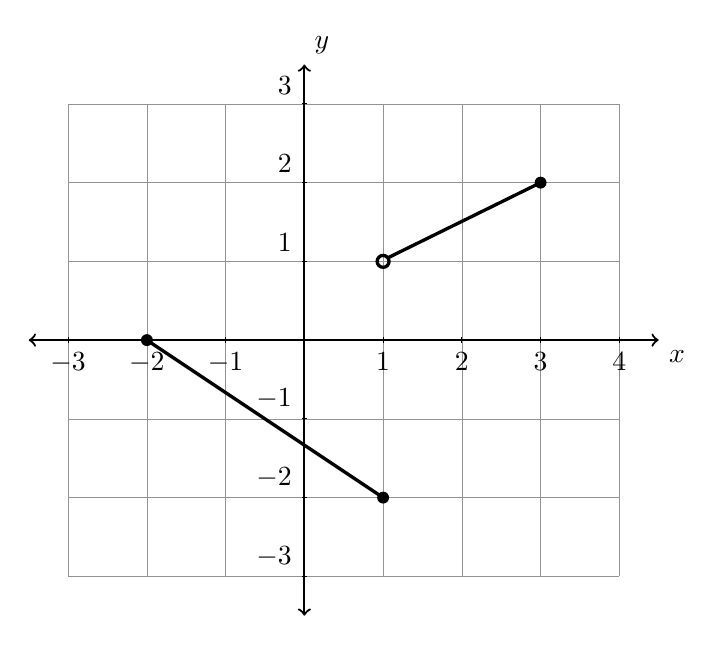
\begin{tikzpicture}[y=1.0cm, x=1.0cm,font=\sffamily,
  mydot/.style={
    circle,
    fill=white,
    draw,
    outer sep=0pt,
    inner sep=1.5pt
  }]
    %% Add a grid
    \draw[step = 1, gray, very thin,opacity=0.85] (-3, -3) grid ( 4, 3);
 	%% Draw the axes
	\draw[thick,<->] (-3.5,0) -- coordinate (x axis mid) (4.5,0) node[anchor = north west] {$x$};
    \draw[thick,<->] (0,-3.5) -- coordinate (y axis mid) (0,3.5) node[anchor = south west] {$y$};
    %% Label the y axis
    \foreach \y in {-3,-2,-1,1,2,...,3} {
      \draw (1pt, \y) -- (-1pt, \y) node[anchor = south east] {$\y$};
    }
    %% Label the x axis
    \foreach \x in {-3,...,-1,1,2,...,4} {
      \draw (\x,1pt) -- (\x,-1pt) node[anchor = north] {$\x$};
    }
    %% Draw the function.
    \begin{scope}
         \draw[scale=1.0,very thick,black] (-2, 0) -- (1,-2);
         \draw[scale=1.0,very thick,black] (1.05,1.04) -- (3,2);
         \fill[black] (-2, 0) circle[radius=0.5ex];
         \fill[black] (3,2) circle[radius=0.5ex];
         \fill[black] (1,-2) circle[radius=0.5ex];
         \draw[scale=1.0, very thick, black] (1,1) circle[radius=0.5ex];

    \end{scope}

    %%\node[above=0.1cm] at (-2,2 )   {\nextXValue};

  \end{tikzpicture}
\end{center}

\vfill

\item
\begin{center}
	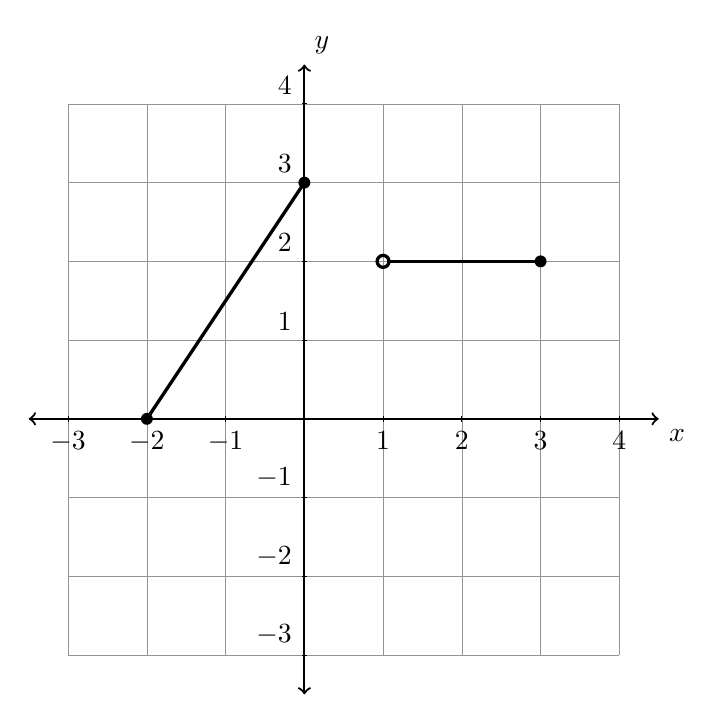
\begin{tikzpicture}[y=1.0cm, x=1.0cm,font=\sffamily,
  mydot/.style={
    circle,
    fill=white,
    draw,
    outer sep=0pt,
    inner sep=1.5pt
  }]
    %% Add a grid
    \draw[step = 1, gray, very thin,opacity=0.85] (-3, -3) grid ( 4, 4);
 	%% Draw the axes
	\draw[thick,<->] (-3.5,0) -- coordinate (x axis mid) (4.5,0) node[anchor = north west] {$x$};
    \draw[thick,<->] (0,-3.5) -- coordinate (y axis mid) (0,4.5) node[anchor = south west] {$y$};
    %% Label the y axis
    \foreach \y in {-3,-2,-1,1,2,...,3,4} {
      \draw (1pt, \y) -- (-1pt, \y) node[anchor = south east] {$\y$};
    }
    %% Label the x axis
    \foreach \x in {-3,...,-1,1,2,...,4} {
      \draw (\x,1pt) -- (\x,-1pt) node[anchor = north] {$\x$};
    }
    %% Draw the function.
    \begin{scope}
         \draw[scale=1.0,very thick,black] (-2, 0) -- (0,3);
         \draw[scale=1.0,very thick,black] (1.05,2) -- (3,2);
         \fill[black] (-2, 0) circle[radius=0.5ex];
         \fill[black] (3,2) circle[radius=0.5ex];
         \fill[black] (0,3) circle[radius=0.5ex];
         \draw[scale=1.0, very thick, black] (1,2) circle[radius=0.5ex];

    \end{scope}

    %%\node[above=0.1cm] at (-2,2 )   {\nextXValue};

  \end{tikzpicture}
\end{center}

\vfill

\end{enumerate}

\clearpage

\item Determine the domain of each of the following functions. Give your answer in interval notation.%\\[.5in]
\begin{enumerate}
\item $g(x) = x^2$
  \vfill
\item $f(x)=\sqrt{3x-7}$
  \vfill
%\item $f(x) = \dfrac{x+3}{x^2-9}$
\item $h(x)=\dfrac{5}{x^2-25}$
  \vfill
\item $f(x) = \sqrt{x^2-4x+3}$
  \sideNote{Make a sketch of the quadratic function without the square
    root first.}
  \vfill
  \vfill
\item $g(x) = \dfrac{\sqrt{x^2-4x+3}}{x^3+8}$
  \vfill

\end{enumerate}

\clearpage

\item The graph of different relationships are given in the figures
  below. For each relationship determine whether or not the
  relationship is a function. Provide specific reasons for your
  conclusion and do not just cite the name of a particular rule or
  test. Also, state all of the intercepts for each relationship.

  \begin{enumerate}
  \item
  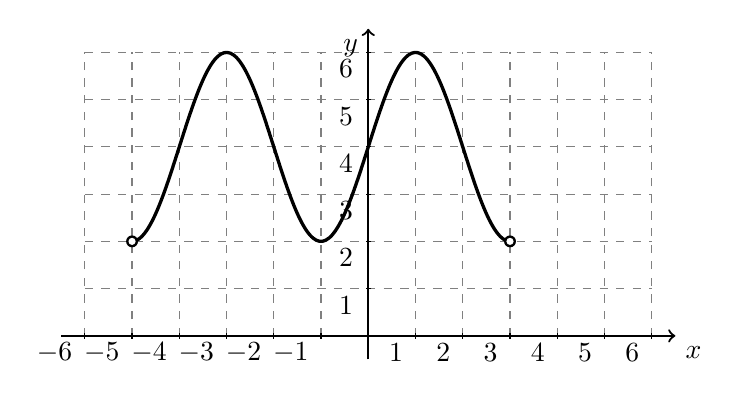
\begin{tikzpicture}[y=0.6cm, x=0.6cm,font=\sffamily]
    %% ticks
    \draw[step = 1, gray,dashed] (-6,0) grid (6,6);
    %% axis
    \draw[thick,->] (-6.5,0) -- coordinate (x axis mid) (6.5,0) node[anchor = north west] {$x$};
    \draw[thick,->] (0,-.5) -- coordinate (y axis mid) (0,6.5) node[anchor = north east] {$y$};
    \foreach \y in {1,2,...,6} {
      \draw (1pt, \y) -- (-1pt, \y) node[yshift=-6,xshift=-1,anchor=east] {$\y$};
    }
    \foreach \x in {-6,-5,...,-1,1,2,...,6} {
      \draw (\x,1pt) -- (\x,-1pt) node[yshift=-5,xshift=-1,anchor=east] {$\x$};
    }

    \begin{scope}
      %\clip(-4,-1) rectangle (8,5);
      \draw[scale=1.0,domain=-4:4,smooth,variable=\x,very thick,black,samples=120] 
           plot ({\x-1},{4+2*sin(deg(pi*\x/2-pi/2))});
      \fill[black] (-5,2) circle [radius=0.5ex];
      \fill[white] (-5,2) circle [radius=0.3ex];
      \fill[black] ( 3,2) circle [radius=0.5ex];
      \fill[white] ( 3,2) circle [radius=0.3ex];
    \end{scope}

  \end{tikzpicture}

  \item 
    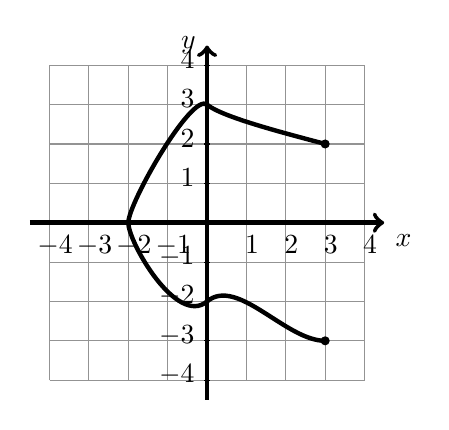
\begin{tikzpicture}[y=0.5cm, x=0.5cm,font=\sffamily]
      \draw[step = 1, gray, thin,opacity=0.85] (-4,-4) grid (4,4);
      \draw[black,ultra thick,->] (-4.5,0) -- (4.5,0) node[anchor=north west] {$x$};
      \draw[black,ultra thick,->] (0,-4.5) -- (0,4.5) node[anchor=east] {$y$};
      \foreach \y in {-4,-3,-2,-1,1,2,3,4} {
        \draw (1pt, \y) -- (-1pt, \y) node[anchor = east,yshift=2] {$\y$};
        \draw (\y,1pt) -- (\y,-1pt) node[anchor = north,xshift=2] {$\y$};
      }
      \draw[ultra thick,black] (3, -3) .. controls +(0:-1) and +(40:1) .. (0, -2)
                    ( 0,-2) .. controls +( 40:-1.0) and +(90:-0.5) .. (-2, 0)
                    (-2, 0) .. controls +( 90:0.5) and +(-40:-0.5) .. (0,3)
                    ( 0, 3) .. controls +(-40:0.5) and +(-15:-1) .. (3, 2);
          \draw[black,fill=black]  (3,-3) circle (0.1);
          \draw[black,fill=black]  (3, 2) circle (0.1);

    \end{tikzpicture}
  \end{enumerate}
  
  \clearpage


\end{enumerate}

\hwTitle{Homework Section 1.3}

\begin{enumerate}
\item The Racine express is moving straight North out of Chicago at a
  speed of 80 kilometers per hour. The Davenport Traveler is moving
  straight West out of Chicago at a speed of 90 kilometers per
  hour. The trains leave the station at the same time. Determine an
  equation for the distance between the two trains as a function of
  time.

\item Consider the relation that is defined by taking an object on
  your desk and assigning to it its color.  For example, if there is a
  hat on your desk that is green and blue, we would write
  $$f(\text{hat}) = \{\text{green, blue}\}.$$
  If there is a pen on your desk that is red, we would write
  $$f(\text{pen}) = \text{red}.$$
\begin{enumerate}
\item List at least three items on your desk and come up with your own
  relation. (You can use imaginary items or objects in the room, if
  you need to.)
\item What is the domain and range of your relation?
\item Is your relation a function?  Why or why not?
\end{enumerate}

\item Determine the domain of each of the following functions. Give your answer in interval notation.%\\[.5in]
\begin{enumerate}
\item $g(x) = x^3$
\item $f(x)=\sqrt{x+1}$
\item $h(x)=\frac{5}{x-4}$
\item $k(x) = \dfrac{x+3}{x^2-9}$
\item $l(x)=\dfrac{1}{x^2+1}$
\item $m(x) = \sqrt{x^2-2x-15}$
\item $n(x) = \frac{1}{\sqrt{x^2-2x-15}}$
\end{enumerate}

\item Use the axes below to make a rough sketch of each of the
  indicated functions.
  \pagebreak[4]
  \begin{enumerate}

  \item ${\displaystyle y=x^2}$
\begin{center}
	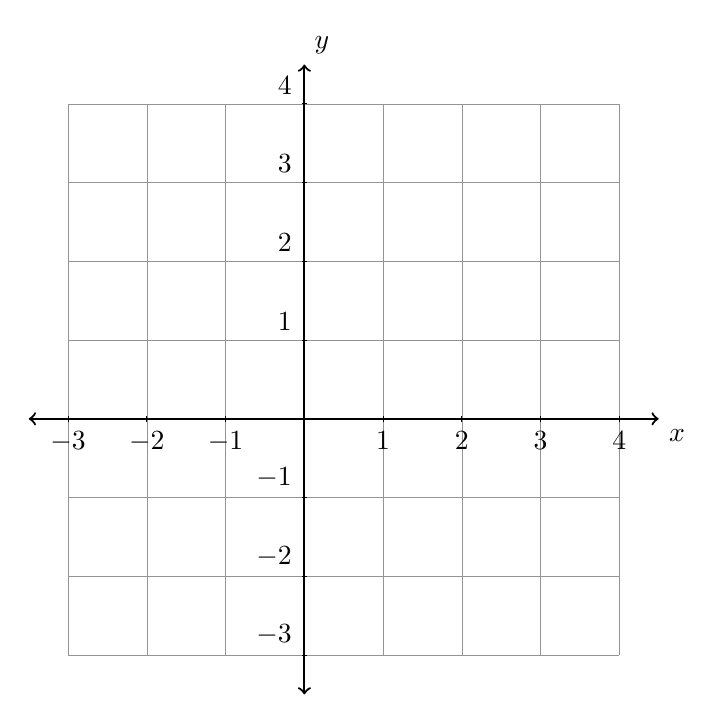
\begin{tikzpicture}[y=1.0cm, x=1.0cm,font=\sffamily,
  mydot/.style={
    circle,
    fill=white,
    draw,
    outer sep=0pt,
    inner sep=1.5pt
  }]
    %% Add a grid
    \draw[step = 1, gray, very thin,opacity=0.85] (-3, -3) grid ( 4, 4);
 	%% Draw the axes
	\draw[thick,<->] (-3.5,0) -- coordinate (x axis mid) (4.5,0) node[anchor = north west] {$x$};
    \draw[thick,<->] (0,-3.5) -- coordinate (y axis mid) (0,4.5) node[anchor = south west] {$y$};
    %% Label the y axis
    \foreach \y in {-3,-2,-1,1,2,...,3,4} {
      \draw (1pt, \y) -- (-1pt, \y) node[anchor = south east] {$\y$};
    }
    %% Label the x axis
    \foreach \x in {-3,...,-1,1,2,...,4} {
      \draw (\x,1pt) -- (\x,-1pt) node[anchor = north] {$\x$};
    }
  \end{tikzpicture}
\end{center}

\item ${\displaystyle y=x}$
\begin{center}
	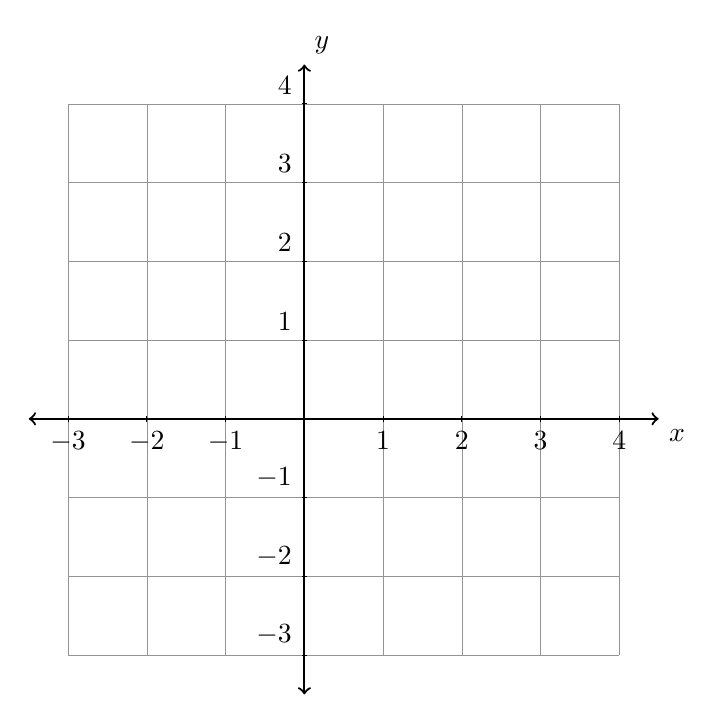
\begin{tikzpicture}[y=1.0cm, x=1.0cm,font=\sffamily,
  mydot/.style={
    circle,
    fill=white,
    draw,
    outer sep=0pt,
    inner sep=1.5pt
  }]
    %% Add a grid
    \draw[step = 1, gray, very thin,opacity=0.85] (-3, -3) grid ( 4, 4);
 	%% Draw the axes
	\draw[thick,<->] (-3.5,0) -- coordinate (x axis mid) (4.5,0) node[anchor = north west] {$x$};
    \draw[thick,<->] (0,-3.5) -- coordinate (y axis mid) (0,4.5) node[anchor = south west] {$y$};
    %% Label the y axis
    \foreach \y in {-3,-2,-1,1,2,...,3,4} {
      \draw (1pt, \y) -- (-1pt, \y) node[anchor = south east] {$\y$};
    }
    %% Label the x axis
    \foreach \x in {-3,...,-1,1,2,...,4} {
      \draw (\x,1pt) -- (\x,-1pt) node[anchor = north] {$\x$};
    }
  \end{tikzpicture}
\end{center}

\pagebreak[4]

\item ${\displaystyle y=\sqrt{x}}$ 
\begin{center}
	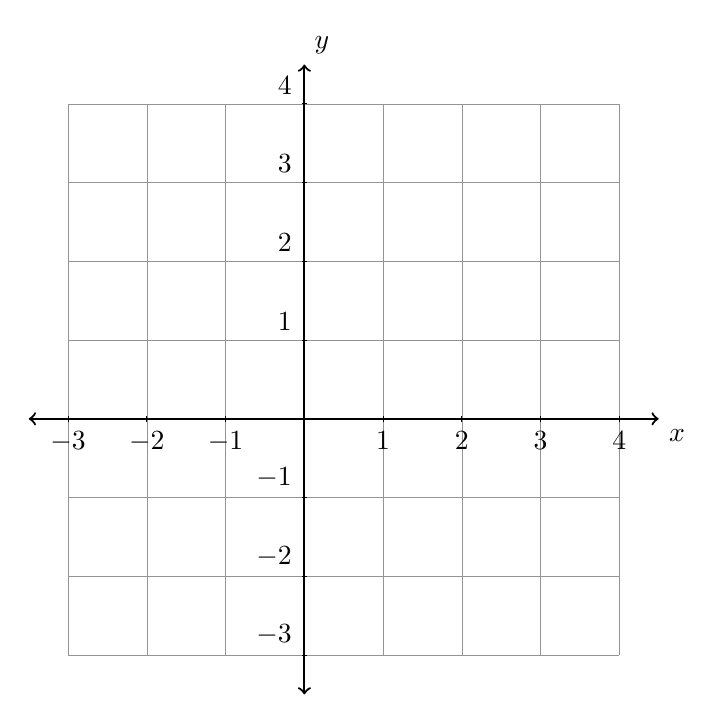
\begin{tikzpicture}[y=1.0cm, x=1.0cm,font=\sffamily,
  mydot/.style={
    circle,
    fill=white,
    draw,
    outer sep=0pt,
    inner sep=1.5pt
  }]
    %% Add a grid
    \draw[step = 1, gray, very thin,opacity=0.85] (-3, -3) grid ( 4, 4);
 	%% Draw the axes
	\draw[thick,<->] (-3.5,0) -- coordinate (x axis mid) (4.5,0) node[anchor = north west] {$x$};
    \draw[thick,<->] (0,-3.5) -- coordinate (y axis mid) (0,4.5) node[anchor = south west] {$y$};
    %% Label the y axis
    \foreach \y in {-3,-2,-1,1,2,...,3,4} {
      \draw (1pt, \y) -- (-1pt, \y) node[anchor = south east] {$\y$};
    }
    %% Label the x axis
    \foreach \x in {-3,...,-1,1,2,...,4} {
      \draw (\x,1pt) -- (\x,-1pt) node[anchor = north] {$\x$};
    }
  \end{tikzpicture}
\end{center}

\item ${\displaystyle y=\frac{1}{x}}$
  \nopagebreak[4]
\begin{center}
	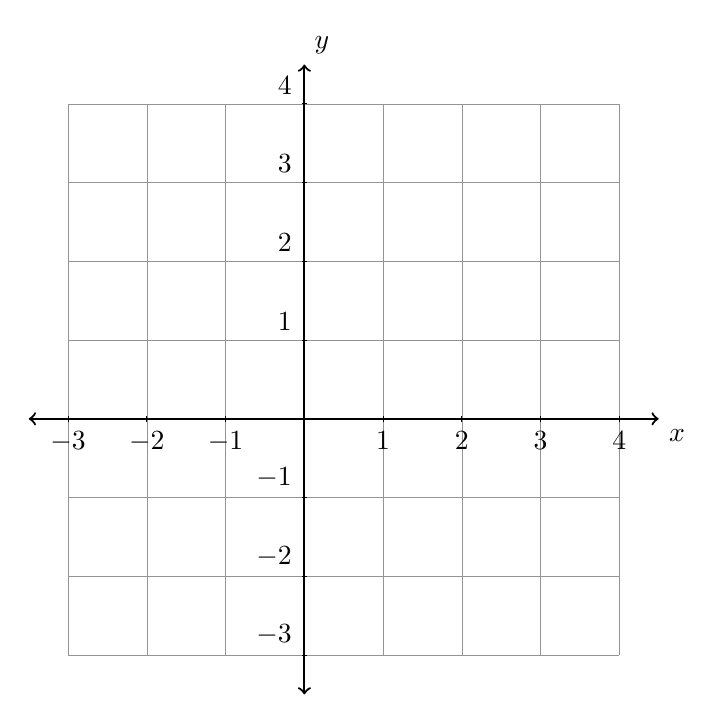
\begin{tikzpicture}[y=1.0cm, x=1.0cm,font=\sffamily,
  mydot/.style={
    circle,
    fill=white,
    draw,
    outer sep=0pt,
    inner sep=1.5pt
  }]
    %% Add a grid
    \draw[step = 1, gray, very thin,opacity=0.85] (-3, -3) grid ( 4, 4);
 	%% Draw the axes
	\draw[thick,<->] (-3.5,0) -- coordinate (x axis mid) (4.5,0) node[anchor = north west] {$x$};
    \draw[thick,<->] (0,-3.5) -- coordinate (y axis mid) (0,4.5) node[anchor = south west] {$y$};
    %% Label the y axis
    \foreach \y in {-3,-2,-1,1,2,...,3,4} {
      \draw (1pt, \y) -- (-1pt, \y) node[anchor = south east] {$\y$};
    }
    %% Label the x axis
    \foreach \x in {-3,...,-1,1,2,...,4} {
      \draw (\x,1pt) -- (\x,-1pt) node[anchor = north] {$\x$};
    }
  \end{tikzpicture}
\end{center}

\end{enumerate}




\end{enumerate}
